\section{Phase 4 - Making a demo}

At this point in the development we were sure about what kind of situation we wanted to simulate to make a satisfying product for Accenture, and to answer the problem statement we had decided on. Following the work requirements we now needed to make a demonstration that showed how the system worked. At this point we also decided that we wanted to make a physical demonstration instead of making a digital simulation, although this was a solution that would take less effort and still be a valid solution. At the start of this work phase we had started to consider making only a digital simulation, but after a meeting with our external supervisors at Accenture, in which we were advised that a physical demonstration was more in line with Accenture's goals for the project, we finally decided to make a physical demonstration. 

\subsection{Building a new car}
The previous group had only built one car for their project. Consequently, we needed to build a new car to show a situation where two cars meet at an intersection. Luckily, Accenture kept a box of unused components from the previous group. However, we only had one TPU, the Coral Usb Accelerator. The TPU is an essential component for giving extra processing power to the computer, and it was necessary to run the artificial intelligence the previous group had used \parencite{prev_project}. 

Without this accelerator, we could not run the artificial intelligence the previous group had incorporated into their solution due to the global chip shortage caused by the Covid pandemic; the accelerator was unavailable to purchase anywhere. As a result, the new car's camera and distance measuring sensor were absent. Not having two cars that utilized artificial intelligence could be a challenge. One of the required features of our solution was that the cars should be able to drive using the AI when a server connection was unavailable, as per described in \secref{sec:goals}. We decided that as long as we had one car that could navigate traffic independent of the server, the other car could drive solely on commands given by the server. With the components and the product documentation of the previous project \secref{sec:goals}, we were able to build a copy of the car as seen in \figref{fig:twocars}.

\begin{figure}[h!]
	\centering
	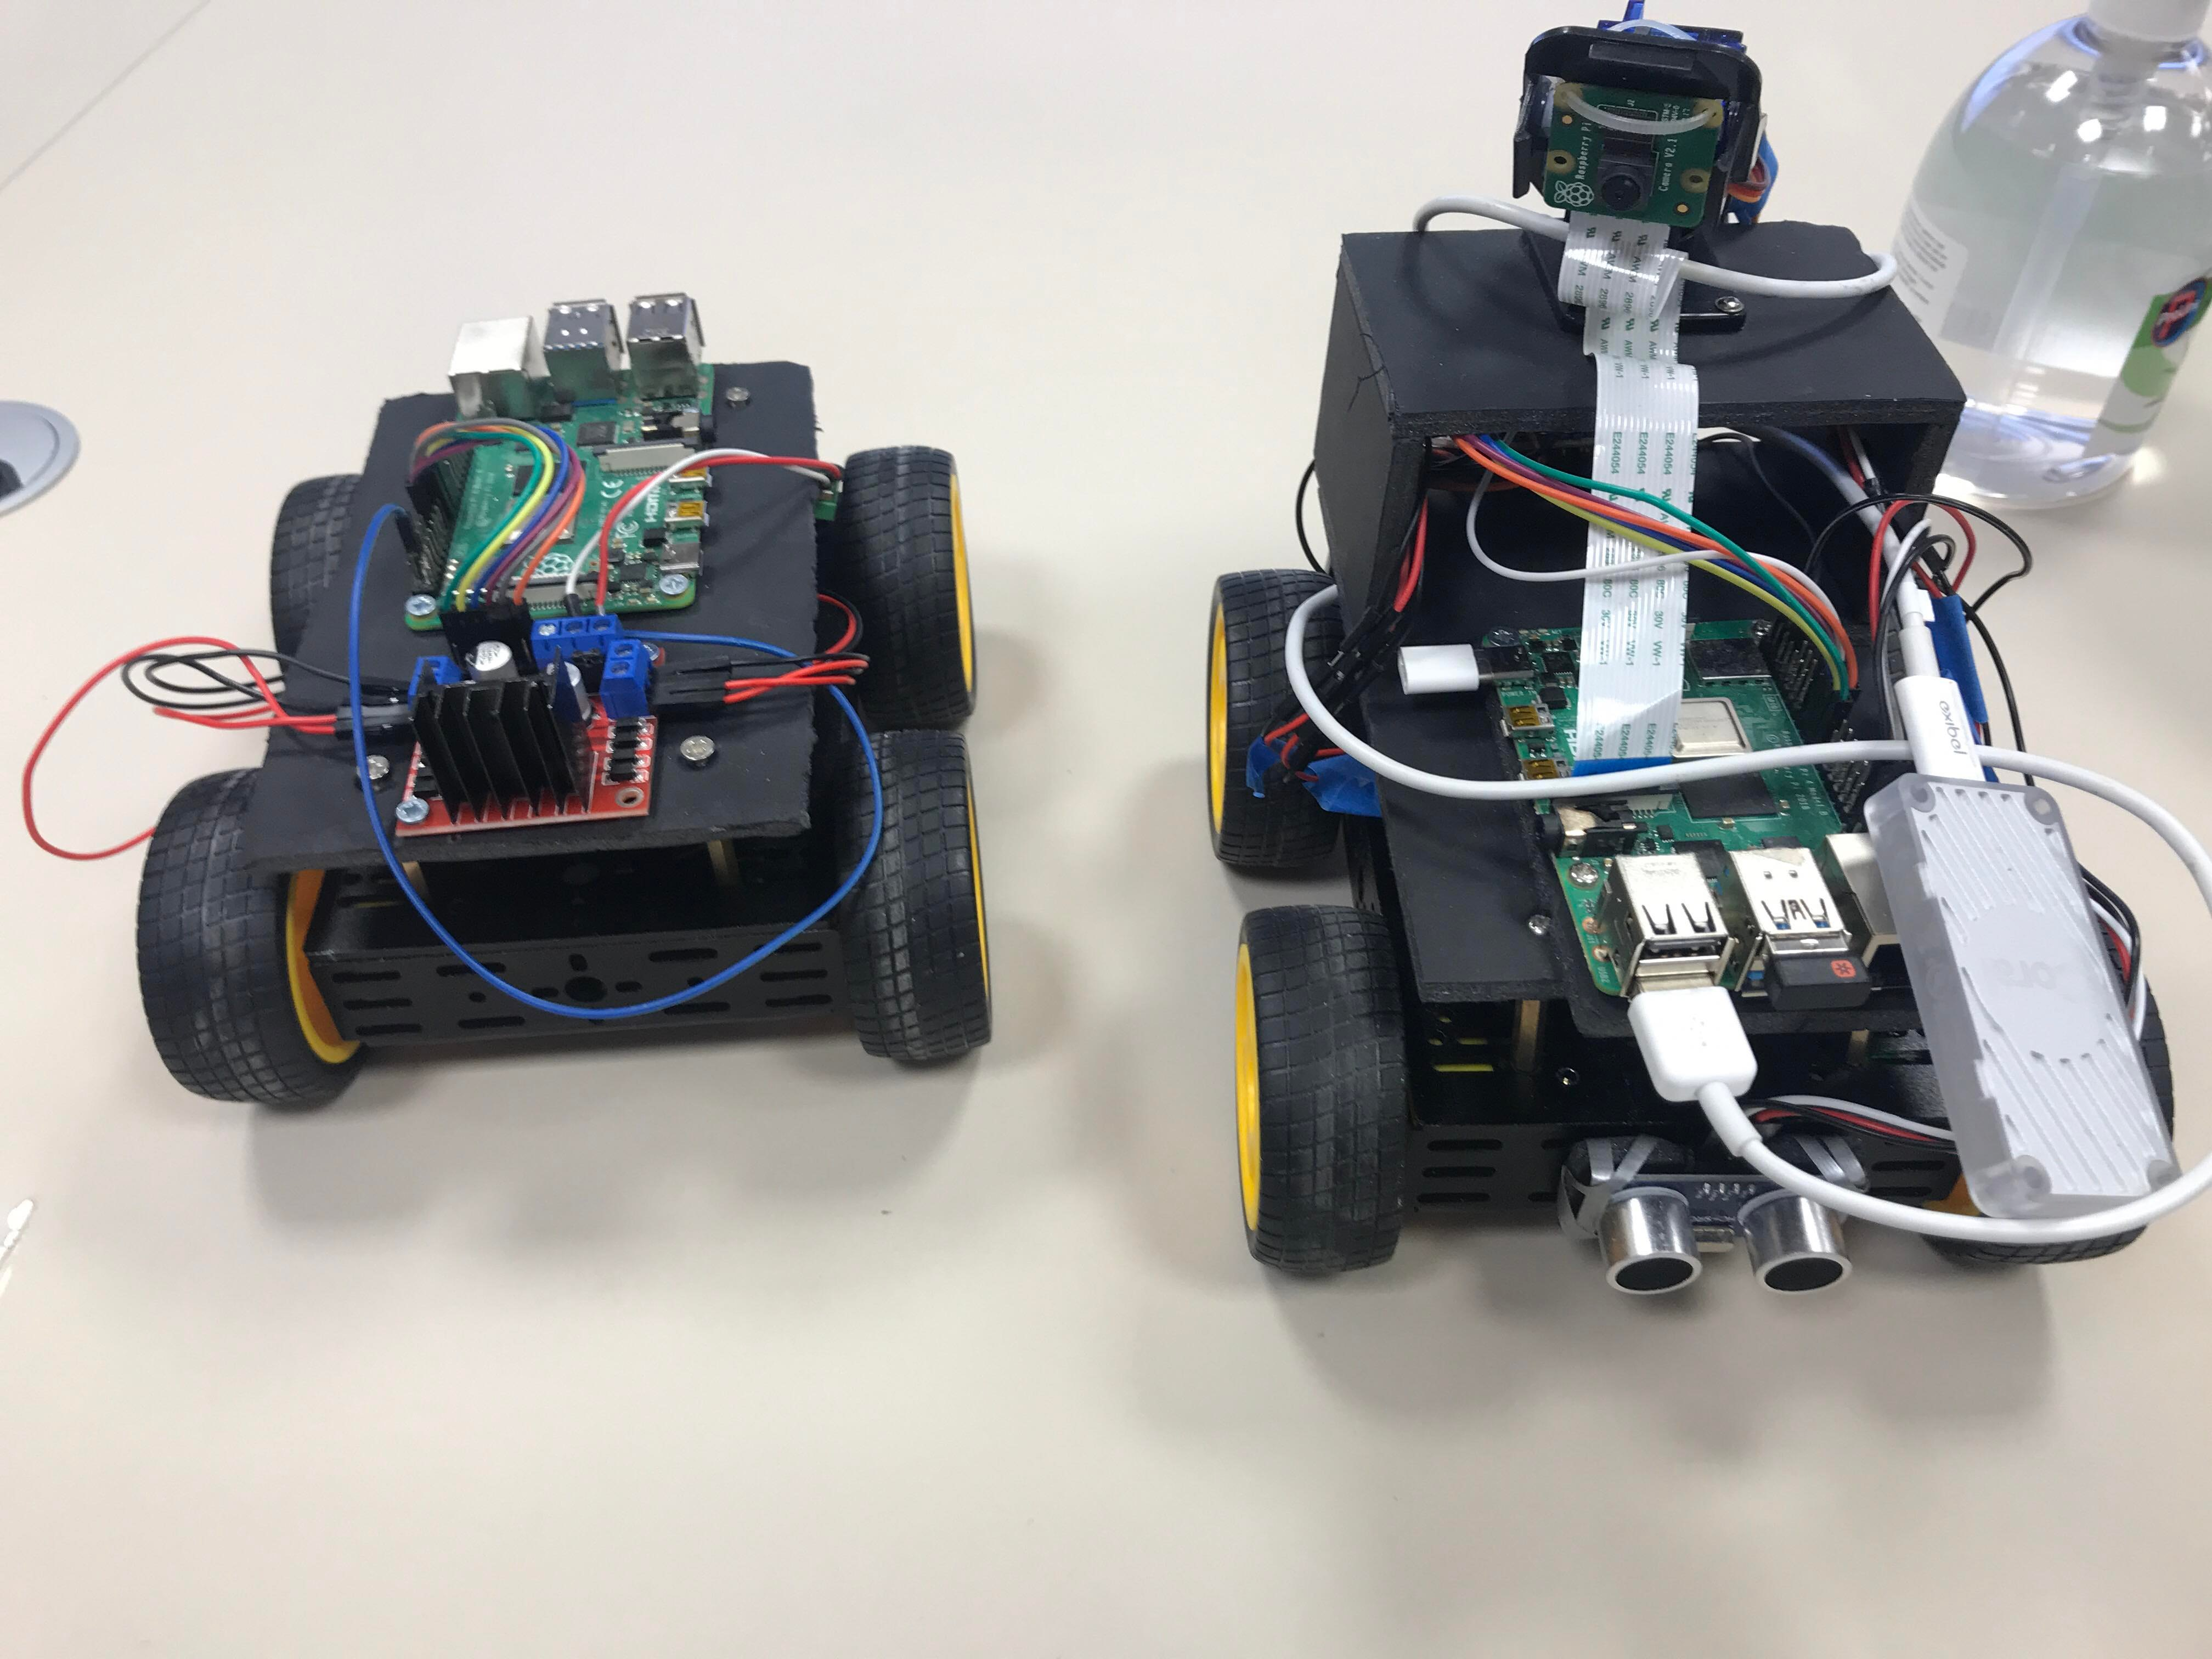
\includegraphics[width=0.9\linewidth]{figures/two_cars}
	\caption{Photo of the two cars we built. To the left is the car without a camera. To the right is the car with a camera on top and a Coral USB Accelerator Edge TPU. This car can take advantage of the onboard AI.}
	\label{fig:twocars}
\end{figure}




\subsection{Calibration of the cars}
When the server, vehicles and client were implemented, and the second vehicle built, we did some testing to figure out how the car’s behaved when given directions by the server. In this test the vehicles were given a specific velocity and driving distance by the server. When the vehicles arrived at their destination the server would tell them to stop. The car’s drove in a straight line.

The vehicles were able to send information, and respond correctly to the servers commands. We also observed that the vehicles drove a different length for each velocity given even though the length was the same. This is because the velocity given to the vehicles is the amount of power going into the car’s motors, not the actual velocity of the car’s. We wanted the demo to be accurate so our group did some further testing where we wrote down the results. 

\begin{table}
	\begin{center}
		\begin{tabular}{rrrr}
			\hline
			Power (?) & Length (cm) & Time (s) & Velocity (cm/s) \\
			\hline
			40 & 467 & 8.98 & 52.00 \\
			50 & 425 & 7.28 & 58.38 \\
			60 & 400 & 6.06 & 66.01 \\
			70 & 357 & 5.18 & 68.92 \\
			80 & 325 & 4.49 & 72.32 \\
			90 & 314 & 4.03 & 77.92 \\
			100 & 286 & 3.62 & 79.01 \\
			\hline
		\end{tabular}
		\caption{Test text}
	\end{center}
\end{table}

The data Power was the velocity given by the server. Velocity was the actual velocity in our testing, which is length divided by time. As you can see the velocity was not the same as the power. We then made a graph to visualize the two values. The $y$-axis was the velocity while the $x$-axis is the power.

\begin{figure}[h!]
	\caption{Graph of velocity as a function of power}
\end{figure}

We observed that the correlation between power and velocity seemed linear. This means we could make a specific formula that describes the correlation between the two values. We used linear regression to figure out this formula:

\begin{figure}[h!]
	\caption{Graph of velocity as a function of power with linear regression}
\end{figure}

The formula we ended up with was as follows: $P = 0.4516v + 36.189$, where $P$ is power and $v$ is velocity, with a mean square error of $R^2=0.9653$. When we coded the formula into the vehicles we did another set of testing. We observed that the vehicles drove more or less the same distance for each power given. If we wanted an even more accurate formula we could have tuned the formula with the test results from our new test. Although the results were not hundred percent accurate, we concluded it was accurate enough for our demonstration. 

To test the solution we have worked on, we made a physical demonstration with two cars that meet at an intersection, as part of the product documentation. We want to test that a combination of a centralized communication system and artificial intelligence can improve traffic flow. What we wanted to observe was if the velocity of the vehicles were not drasticly changed and therefore not distrupting the traffic flow.


\subsection{Construction of semi physical demonstration}\label{sec:demo}
We wanted to test that a centralized communication system and artificial intelligence could improve traffic flow. In order to test the solution, we made a semi physical simulation where two cars approach an intersection simultaneously. We wanted to observe if the velocity of the vehicles were not drastically changed and, therefore, decreased shockwave described in \secref{sec:traffic_congestion}.

We found a space at Accenture that was big enough to build the track. The power input on the Raspberry Pi vehicles is limited to between 40 and 100 units. Since the server will adjust the vehicle's speed to avoid a collision, the intersection was required to be at least 130cm away from the starting point to prevent the server from adjusting speed outside the equivalent power limit. Furthermore, the server prevents cars from driving before at least two vehicles have established a connection. Hence, both vehicles will start their journey simultaneously. We also placed the vehicles at the same distance from the intersection on their respective roads. Given these initial conditions, both vehicles are supposed to collide without the server's intervention. We also made the server log the velocity sent to the cars to track how much the cars' velocities changed.

Making the demo one hundred percent accurate was not possible in our circumstances due to the limitations of the Raspberry Pi. Furthermore, the vehicles were not able to receive the messages simultaneously. Consequently, this meant that they could start with a minor time difference. Another factor was that the trajectory of the vehicles was not always straight. However, we were able to get a consistent demo with enough margins. \figref{fig:crashdemo} shows an example of a collision during a test demonstration.

\begin{figure}[h!]
	\centering
	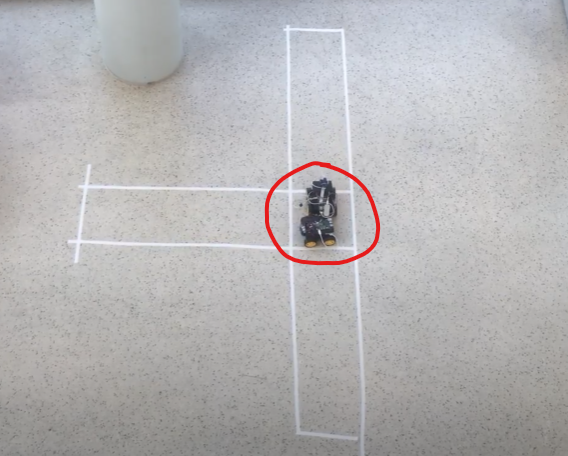
\includegraphics[width=1\linewidth]{figures/demo_crash}
	\caption{Here, we can observe the two cars colliding in the intersection. One of the cars started about 5 centimeters further behind the other car and started a few milliseconds later, resulting in a collision. Meanwhile, the server assumed they started simultaneously at the same distance from the intersection.}
	\label{fig:crashdemo}
\end{figure}

Furthermore, the server did not account for the lengths of the vehicles during its calculations. After we introduced the length of the vehicles and buffer zone, we were able to get a consistent semi-physical demonstration.

When both vehicles had connected to the server, the cars would drive with an initial speed of 80 cm/s, the upper limit of the Raspberry Pi. Not long after they started to drive, the server recognized the cars approaching the intersection. The server calculates using the car's velocity, position, and length. Then the server calculates which car has to slow down and how much the car needs to slow down to avoid a collision, in this case, to 55 cm/s. After the other car has supposedly passed the intersection, the car that slowed down gets told by the server to speed its velocity back to 80 cm/s. \figref{fig:successdemo} is a snapshot of a successful test demo.

\begin{figure}[h!]
	\centering
	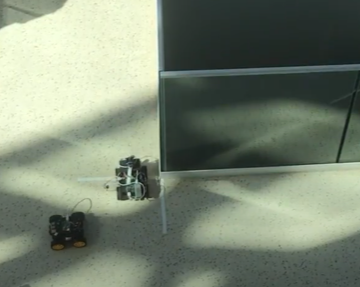
\includegraphics[width=1\linewidth]{figures/succsess_demo}
	\caption[Successful demo]{Here is a snipped from a successful demo. The car to the left has just passed the intersection, marked as a square with white tape. The car furthest up is, therefore, about to adjust back to its original velocity. Here we can observe that the server prevents a collision.}
	\label{fig:successdemo}
\end{figure}
%\input{chapters/sections/subsections/building_road_model}
%\input{chapters/sections/subsections/simulating_situation}

